% Canonical integrated PRE manuscript. The legacy builder requires --force-legacy.
\documentclass[aps,pre,twocolumn,superscriptaddress,floatfix,nofootinbib]{revtex4-2}

\usepackage{amsmath,amssymb,amsthm,bm}
\usepackage{graphicx}
\usepackage[colorlinks=true,allcolors=blue]{hyperref}

\newcommand{\eps}{\varepsilon}
\newcommand{\epst}{\tilde{\eps}}
\newcommand{\avg}[1]{\left\langle #1 \right\rangle}
\newcommand{\Teff}{T_{\mathrm{eff}}}
\newcommand{\Var}{\mathrm{Var}}
\newcommand{\dd}{\mathrm{d}}
\newtheorem{proposition}{Proposition}
\newtheorem{remark}{Remark}

\begin{document}
\title{Temporal Organization Amplifies Counting Fluctuations in Signed Order Flow}

\author{Nelson Bol\'{\i}var}
\affiliation{Escuela de F\'{\i}sica, Facultad de Ciencias, Universidad Central de Venezuela, Caracas 1041-A, Venezuela}
\affiliation{Astrum Drive Technologies, 13024 Dallas Pkwy Unit 120 B, Frisco, TX 75034, USA}
\author{Gabriel Abell\'an}
\affiliation{Escuela de F\'{\i}sica, Facultad de Ciencias, Universidad Central de Venezuela, Caracas 1041-A, Venezuela}
\affiliation{Astrum Drive Technologies, 13024 Dallas Pkwy Unit 120 B, Frisco, TX 75034, USA}
\author{David Verrilli}
\affiliation{Escuela de F\'{\i}sica, Facultad de Ciencias, Universidad Central de Venezuela, Caracas 1041-A, Venezuela}
\date{\today}

\begin{abstract}
Temporal organisation changes how signed market-order flow accumulates. We
measure that change as a counting-statistics problem in four cryptocurrency
markets over four years, with four additional assets used for post-hoc
robustness of the central comparison and broader panels reserved for labelled
diagnostic tests. A calendar-matched permutation null preserves transfer sizes and
one-point statistics while destroying chronology; the observed weekly
variance exceeds this null for both raw and normalised flow. An exact identity,
with the recentring correction required by the operational null, then
separates the variance into transfer-size, sign-memory, and sign--size cross
terms. Within the excess over the size baseline, the corrected cross
contribution exceeds the sign-memory contribution in all eight primary point
estimates, while paired bootstrap intervals resolve a majority share in six.
Drift-resistant estimators give finite-window superdiffusive exponents
$1.10$--$1.36$, without identifying an asymptotic exponent. Additional
diagnostics delimit, rather than enlarge, this result: a linear fluctuation
symmetry has a Gaussian explanation and an apparent post-shock clock is
reproduced by randomly placed events. The central finding is the
null-controlled amplification and its exact sign--size decomposition.
\end{abstract}
\maketitle

\section{Introduction}

Signed order flow is persistent, but persistence alone does not determine how
much net volume accumulates over a finite interval. Transfer sizes are
heterogeneous and clustered, signs are long-memory variables, and their joint
ordering can contribute even when neither marginal statistic changes. Our
central result isolates that joint contribution. In four years of
cryptocurrency data, weekly counting variance exceeds a calendar-matched
memoryless baseline. An exact decomposition aligned with that null then shows
that, within the excess over the size baseline, the sign--size cross
contribution exceeds the sign-memory contribution in all eight primary point
estimates, with a majority share statistically resolved in six. The result is
therefore an exact algebraic partition with explicitly limited statistical
scope, not a causal attribution or a claim that one mechanism dominates every
market.

Long-memory order signs and finite-window superdiffusive accumulated flow are established
features of market microstructure \cite{lillo2004,lillo2005,sato2023prl,
sato2023prr}. Maitrier and Bouchaud \cite{maitrier2026} study moments of the
generalised imbalance $I_T^{\,a}=\sum_t\eps_t q_t^{\,a}$ and their relation to
metaorder impact and volatility, including the $a=1$ observable used here.
Their framework does not supply a calendar-matched null or an attribution of a
fixed-window variance to one-point statistics, sign memory, and their temporal
pairing. Those are the narrower questions addressed here. We define ``temporal
organisation'' as the joint chronological structure that remains after the
declared null preserves transfer sizes, calendar strata, and one-point
statistics. An exact algebraic partition then has its per-stratum reference and
recentering correction fixed by that null.

We use transport language operationally. The accumulated signed flow is a
counted transfer, its lagged covariance with price is a response, and its
autocorrelation fixes its second counting cumulant. This correspondence does
not make the flow a conserved electric charge, the impact a conductance, or
the fitted log-ratio a thermodynamic force. Field-theoretic treatments of
markets and order books already exist \cite{rosaclot1999,shi2021}, as do
effective-temperature and fluctuation-relation constructions
\cite{yura2014,ramezani2025,li2024entropy,gao2026,maskawa2025}. Our use of a
classical doubled-field representation is narrower: it records which
second-order relations follow once the empirical memory kernel and innovation
coupling are specified. In particular, it prevents a Gaussian fluctuation
symmetry or a reconstructed variance from being counted as independent
evidence.

The evidential hierarchy is fixed throughout the article. The temporal-null
excess and the algebraic decomposition are the main measurements. Finite-window
superdiffusive scaling is robust under estimators that remove polynomial drift,
but no asymptotic exponent is claimed. Supplemental diagnostics test tempting
interpretations of the same data; none is used as independent evidence for the
central result.

Cryptocurrency provides public taker-side volume, uninterrupted trading, and
records long enough for weekly counting statistics. The price of that access
is limited generality: the primary claims concern four pairs on one venue, and
additional panels enter only the explicitly labelled robustness and
confirmation tests. We first define the observable and its measured memory.
We then introduce the temporal null, derive the exact decomposition, and test
the finite-window scaling. The conclusion separates established results from
scope limits; supplementary material documents the ancillary controls.

\subsection*{A dictionary between market microstructure and transport}

The translation used in this paper is operational rather than metaphorical:
each transport term names a quantity that can be computed from the market
record. Table~\ref{tab:dictionary} also states where the analogy stops. A
physicist should not infer an entropy current or a fermionic exclusion principle
from the word ``current''; a finance reader should not read the measured
response as a causal metaorder-impact curve.

\begin{table*}[t]
\caption{Operational dictionary. The middle column gives the transport name;
the final column states the interpretation supported by the measurement.}
\label{tab:dictionary}
\begin{ruledtabular}
\begin{tabular}{p{0.24\textwidth}p{0.20\textwidth}p{0.49\textwidth}}
Market quantity & Transport language & Meaning and limit \\
\colrule
Signed taker volume $\eps_t$ & Instantaneous current & Buyer-initiated minus seller-initiated executed volume in one candle. It is an aggregate market observable, not electric charge or entropy production. \\
$Q_T=\sum_{t=1}^{T}\eps_t$ & Transferred charge & Net signed volume accumulated over a declared window. It permits counting statistics, but no conservation law for a closed physical device is assumed. \\
$C_\eps(\tau)$ & Current-noise kernel & Temporal memory of signed flow. Its double sum fixes $\Var(Q_T)$ exactly, so these are two views of one second-order object. \\
$R(\tau)$ & Retarded response & Lagged covariance between later price change and present flow. It is an aggregate response diagnostic, not identified causal impact or electrical conductance. \\
$s(Q)=\log[P(Q)/P(-Q)]$ & Fluctuation-symmetry function & A finite-window distributional asymmetry. A linear form is automatic for a Gaussian and is not by itself a fluctuation theorem. \\
$A_T=2\avg{Q_T}/\Var(Q_T)$ & Operational affinity & The Gaussian log-ratio slope. Calling it a thermodynamic force would require stationarity, microreversibility, and an appropriate large-deviation principle, none established here. \\
$\mathcal F$ & Fano factor & Variance relative to a declared transfer-size quantum. Its absolute level depends on the trade-size distribution; observed/null ratios remove that arbitrary quantum. \\
$-C'_\eps/R$ & Formal FDT ratio & A derivative-based diagnostic, not a measured temperature. We derive its model form but make no empirical claim because uncertainty is unresolved. \\
\end{tabular}
\end{ruledtabular}
\end{table*}

The central calculation can be read without transport vocabulary. Each hour
supplies a signed number: positive when taker buyers dominate and negative when
taker sellers dominate. Adding $168$ consecutive hours gives one weekly net
flow. Its variance across weeks is compared with synthetic histories that
retain the same calendar-conditioned values but alter their temporal order.
Repeating the operation after shuffling only signs or only magnitudes asks which
part of that ordering carries the excess. The transport formulation becomes
useful after this statistical question is clear: it supplies the counting
language, exact closures, and a calibrated short-memory benchmark.

Claims are labelled by logical status throughout. A \emph{measurement} is read
from the data and carries an uncertainty or null comparison. A \emph{closure}
is an identity or model consequence and is not independent evidence. A
\emph{benchmark} shows what a specified physical model produces without
asserting that the market is that model. An \emph{open diagnostic} defines a
future test but does not support a present conclusion.

\section{Signed order flow, data, and measured memory}
\label{sec:data}

We use hourly and four-hourly candles for four cryptocurrency pairs (BTC, ETH,
BNB, SOL against USDT) over four years, $35\,063$ hourly and $8\,766$
four-hourly observations per asset. We declare two observables and carry both
through the memory analysis: raw signed base volume
$\eps_t^{(r)}=2V^{\rm taker\,buy}_t-V_t$ and dimensionless imbalance
$\eps_t^{(n)}=\eps_t^{(r)}/V_t$ (set to zero for a zero-volume candle). The
earlier correlation and scaling figures use $\eps^{(n)}$; every result below
states which definition it uses. No proprietary data is required. Analysis
code, numerical outputs, and data provenance are available
\cite{code_keldysh_finance}.

For the central weekly-null result only, we add hourly XRP, ADA, DOGE, and AVAX
as a post-hoc robustness panel selected before inspecting their decomposition
outcomes. They test cross-asset generality but do not enter the original
all-assets decision rule or the response and scaling fits below.

The weekly-artifact analysis uses a separate exploratory panel of twenty
assets, including the eight above, and its pre-registered confirmation test
uses twenty-nine new assets. These broader panels are reported only as
supplementary cross-memory diagnostics; they do not enlarge the primary sample
retroactively.

In microstructure terms, a taker removes resting liquidity: a buyer-initiated
trade executes against an ask and a seller-initiated trade against a bid. The
candle records their aggregate volumes, not the sign and size of every
individual trade. Accordingly, $\eps^{(r)}$ is a signed volume imbalance and
$\eps^{(n)}\in[-1,1]$ is the fraction of that candle's volume imbalance; neither
is a sequence of individually identified market orders.

We validate the candle construction against public individual-trade archives
for one complete UTC day. The sample contains $9{,}797{,}860$ BTCUSDT and
$4{,}969{,}357$ ETHUSDT trades. Aggregation reproduces each hourly base volume,
taker-buy base volume, and trade count exactly up to floating-point roundoff.
This sample is used only to calibrate the transfer-size normalisation; it is not
treated as an independent long-memory sample.

Three conventions matter enough to state explicitly.

\emph{Causality.} Every window is trailing. This is the property on which
everything else depends, and we test it directly: perturbing the future of the
series must leave past features numerically unchanged.

\emph{Alignment.} Flow features live on the candle index while returns are
differences of log prices, so the feature of candle $j$ corresponds to return
index $j-1$. Getting this offset wrong introduces look-ahead that no
window-based test detects, because the features do not move --- the labels do.

\emph{Sign of impact.} The impact of $\eps_t$ is already inside the closing
price of candle $t$, so referencing the response to $\log(\text{Close})$
measures the subsequent relaxation and returns a spurious negative impact. We
reference to the opening price.

\paragraph*{A limitation of public data, stated up front.}
Naviglio \textit{et al.}\ \cite{naviglio2025} show that impact estimated from
public market data is systematically distorted: models trained on public flow
produce price paths that rise linearly rather than concavely during execution
and revert too little afterwards, and they trace the problem to a
misattribution of the origin of order-flow autocorrelation. The warning applies
to our data source and we do not claim to evade it. It most directly affects
the quantity we are not estimating. We do not reconstruct
metaorders or measure their impact; we measure the aggregate response of the
price to the aggregate signed flow, together with the noise and counting
statistics of that flow. Those are properties of the public series itself
rather than inferences about hidden parent orders. The distinction matters for
the counting observables below, which involve no impact estimation, and should
temper any reading of a lagged response diagnostic as a metaorder-impact curve.

\subsection{Memory of the flow, and why one exponent is not enough}
\label{sec:acf}

The flow autocorrelation $C_\eps(\tau)$ decays as a power law, and this is the
standard point of contact with the literature: order splitting predicts
long-memory signs \cite{lillo2005}, verified microscopically
\cite{sato2023prl,sato2023prr}. Fitting a single exponent over $60$ lags we
use $C_\eps(\tau)\propto\tau^\gamma$ and obtain
$\gamma = -0.380 \pm 0.052$ (BTC) and $-0.474 \pm 0.052$ (ETH) at hourly
resolution, broadly consistent with the reported $\gamma\approx-0.5$.

That agreement, however, needs a caveat that turns out to organise much of this
paper. \emph{The single exponent is not well defined without declaring the lag
window}, because $C_\eps$ has two regimes. Writing the positive decay exponent
as $a=-\gamma$, so $C_\eps(\tau)\propto\tau^{-a}$, local fits give, for the raw
hourly series,
\begin{equation}
  a_f = 1.00\pm0.15,\; 0.87\pm0.08,\; 0.46\pm0.05,\; 1.72\pm0.23
\end{equation}
over $\tau\in[2,10]$ for BTC, ETH, BNB and SOL respectively, against
\begin{equation}
  a_s = 0.17\pm0.13,\; 0.22\pm0.09,\; 0.29\pm0.05,\; 0.16\pm0.32
\end{equation}
over $\tau\in[10,50]$. The fast regime is steeper than the slow one in all four
assets, though the values themselves vary considerably between assets and the
slow exponents carry large errors. A single-exponent fit over a wide window
returns something in between, which is why quoted values of $\gamma$ are
sensitive to the fitting range.

We checked whether the slow regime is an artefact of daily periodicity: a
periodic mean contributes a
non-decaying term to the autocorrelation and could masquerade as slow memory.
Removing the seasonal component barely moves the slopes (e.g.\ BTC:
$-1.003\to-0.941$ fast, $-0.168\to-0.212$ slow), so daily periodicity does not
explain the slow fitted regime; this control does not exclude other forms of
nonstationarity.

\section{Temporal organisation and counting fluctuations}
\label{sec:counting}

Let $Q_T=\sum_{t=1}^{T}\eps_t$ be the signed flow accumulated over $T$
candles. We first ask what its variance retains when chronology is destroyed
without changing transfer sizes, calendar strata, or one-point statistics.
The difference from that temporal null is the empirical core of the paper.
We then decompose the difference exactly, quantify its sign--size cross term,
and estimate how much of that term independent marginal memories reproduce.

\subsection{A calendar-matched temporal null}
\label{sec:whatdoesnotclose}

The robust remainder is temporal rather than a large absolute number. For
reference we write the Fano normalisation as
\begin{equation}
  \mathcal{F}(T)=\frac{\Var(Q_T)}{\bar q^{\,2}\,\avg{N_T}} ,
  \label{eq:fano}
\end{equation}
where $N_T$ is the number of trades. Candles provide only
$\bar q_{\rm proxy}=\operatorname{median}_t(V_t/N_t)$, a median of hourly mean
sizes, not the median of individual sizes. Under this declared proxy,
$\mathcal F(T{=}1)=905$--$3342$. The trade-level calibration of
Sec.~\ref{sec:data} gives directly measured individual-trade medians smaller by factors $87.5$ (BTC) and
$71.6$ (ETH), so the proxy is conservative for the level. It is not, however,
a memory test: an independent compound-Poisson process already gives
$\mathcal F=\avg{q^2}/\bar q^2$, which can be large under a broad size
distribution.

We isolate temporal dependence by comparing weekly windows with stratified
permutation nulls. Complete Monday--Sunday UTC weeks are demeaned within each
quarter-by-hour-of-week stratum. The primary null permutes the complete signed
flow. Two attribution nulls separately permute its signs while preserving the
magnitude path, or its magnitudes while preserving the sign path; all
surrogates are re-centred in the same strata. Raw signed volume and normalised
imbalance are analysed in parallel (Fig.~\ref{fig:counting}). The joint-null
ratio is $2.2$--$3.4$ for
raw flow and $3.0$--$4.3$ for normalised flow. Destroying sign order leaves
nearly the same ratio, whereas destroying magnitude order lowers it to
$1.7$--$2.2$ and $1.5$--$1.9$, respectively. Read as surrogates, these say that
the preserved sign path recovers more of the weekly variance than the preserved
magnitude path. We deliberately do not stop here, and Sec.~\ref{sec:decomp}
explains why: a signed sum admits no clean per-path surrogate, and the exact
decomposition available instead reaches a different conclusion about where the
excess sits. Moving-block bootstrap intervals over weekly sums quantify
the sampling uncertainty (Supplemental Material \cite{supplement}).

The predeclared all-assets screen
$V_{\rm obs}>2Q_{0.9875}(V_{\rm null})$ failed under its declared raw-flow
quarterly joint null because BNB did not pass. We do not replace that outcome
with the later normalised-flow analysis. Monthly and biweekly strata expose
scale sensitivity, and cross-asset correlations preclude treating the four
assets as independent replications.

The four post-hoc assets reproduce the same ordering. Their joint-null ratios
span $2.08$--$5.67$ for raw flow and $2.83$--$5.64$ for normalised imbalance;
in each asset the sign path retains more of the weekly variance than the
magnitude path. This broadens the empirical panel without rewriting the failed
predeclared gate.

\begin{figure*}[t]
  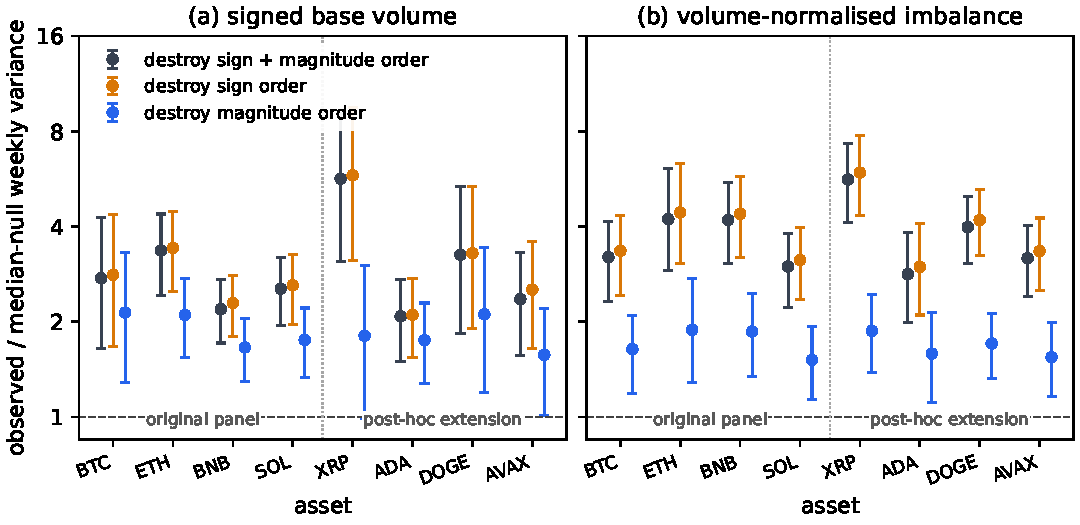
\includegraphics[width=0.98\textwidth]{../output/figuras/fig15_flow_null_decomposition.pdf}
  \caption{Weekly observed/null variance ratios for the joint, sign-order, and
  magnitude-order nulls under both flow definitions. Bars are eight-week
  moving-block bootstrap intervals; the transfer quantum cancels. Every joint
  ratio exceeds one, so the observed chronology carries variance that the
  calendar-matched memoryless histories do not. The two partial nulls motivate,
  but do not replace, the exact decomposition in Table~\ref{tab:decomp}.}
  \label{fig:counting}
\end{figure*}

\subsection{Exact decomposition of the null-controlled excess}
\label{sec:decomp}

The surrogate comparison above has a structural limit that no number of
permutations removes. Writing $\eps_t=s_t m_t$ with $s_t=\operatorname{sign}
\eps_t$ and $m_t=|\eps_t|$, the accumulated flow $Q_w=\sum_{t\in w}s_t m_t$ is a
\emph{signed} sum, so the magnitude path alone fixes no cumulant of $Q_w$
without the signs. A surrogate that permutes one path while holding the other
necessarily destroys the contemporaneous pairing as well, and cannot therefore
attribute variance to a path cleanly. The attribution nulls above are
diagnostics, not a decomposition.

An exact decomposition is available and needs no surrogate. For any constant
$\bar m$, splitting $m_t m_{t'}=\bar m^2+(m_t m_{t'}-\bar m^2)$ and using
$s_t^2=1$ on the diagonal gives
\begin{equation}
  Q_w^2=\underbrace{\sum_{t\in w}m_t^2}_{\rm size}
   +\underbrace{\bar m^{2}\!\!\sum_{t\neq t'\in w}\!\!s_t s_{t'}}_{\rm sign}
   +\underbrace{\sum_{t\neq t'\in w}\!\!s_t s_{t'}
     \bigl(m_t m_{t'}-\bar m^{2}\bigr)}_{\rm cross} ,
  \label{eq:decomp}
\end{equation}
an identity, verified numerically to a relative $5\times10^{-9}$ on our series,
the residual being floating-point cancellation in the subtraction. Candles of
zero volume, where $s_t=0$ and hence $s_t^2\neq1$, are harmless because $m_t=0$
at exactly those positions. Each term costs $O(n)$: $\sum_{t,t'}s_ts_{t'}=
(\sum_t s_t)^2$ and $\sum_{t,t'}s_ts_{t'}m_tm_{t'}=Q_w^2$, so the cross term
follows by subtraction. The size term is the no-memory baseline that
Eq.~\eqref{eq:fano} normalises to, and the excess over it is the sign term plus
the cross term.

\begin{table}[t]
  \caption{Exact decomposition of $\avg{Q_w^2}$ at weekly scale ($T=168$~h)
  with $\bar m_{h(t)}$ taken per stratum (quarter $\times$ hour-of-week), so
  that the three shares sum to one by Eq.~\eqref{eq:decomp} after carrying the
  recentring correction defined in the text. Because the analysed residual is
  centred in the same strata used by the nulls, averaged $D$ and $D{+}S$ equal
  the expected joint- and magnitude-null second moments. The last
  column gives the corrected cross term as a
  fraction of the excess over the size baseline, with $95\%$ \emph{paired}
  intervals from $3999$ circular moving-block bootstrap replicates of length
  eight weeks --- the same block resample applied to $D$, $S$ and $K$ at once
  --- over the $206$ weekly windows.}
  \label{tab:decomp}
  \begin{ruledtabular}
  \begin{tabular}{lcccc}
   & size & sign & cross & cross/excess \\
  \colrule
  BTC (raw)  & 0.367 & 0.103 & 0.531 & 0.838\ [0.657,\,0.934] \\
  ETH (raw)  & 0.299 & 0.178 & 0.523 & 0.746\ [0.646,\,0.840] \\
  BNB (raw)  & 0.458 & 0.145 & 0.397 & 0.732\ [0.570,\,0.913] \\
  SOL (raw)  & 0.395 & 0.176 & 0.429 & 0.708\ [0.592,\,0.804] \\
  \colrule
  BTC (norm.)& 0.315 & 0.297 & 0.389 & 0.567\ [0.483,\,0.656] \\
  ETH (norm.)& 0.238 & 0.293 & 0.470 & 0.616\ [0.525,\,0.682] \\
  BNB (norm.)& 0.240 & 0.298 & 0.463 & 0.608\ [0.549,\,0.677] \\
  SOL (norm.)& 0.336 & 0.324 & 0.340 & 0.511\ [0.364,\,0.623] \\
  \end{tabular}
  \end{ruledtabular}
\end{table}

Table~\ref{tab:decomp} gives the split. Two qualifications must travel with
these numbers, and both follow from the identity rather than from the data.

\paragraph*{$\bar m$ is a free parameter; the operational null fixes the
recentring correction.}
Equation~\eqref{eq:decomp} holds for \emph{any} constant, so the boundary
between the sign and cross terms is in general a convention. The dependence is
exact: for two choices $\bar m_1,\bar m_2$,
\begin{equation}
  {\rm cross}(\bar m_1)={\rm cross}(\bar m_2)
   +\frac{\bar m_2^{2}-\bar m_1^{2}}{\bar m_2^{2}}\,{\rm sign}(\bar m_2) ,
  \label{eq:mbarshift}
\end{equation}
so changing $\bar m$ moves a multiple of the sign term into the cross term and
nothing else, and with a single global $\bar m=\avg{m}$ the cross term is
$0.49$--$0.71$ of the excess. The stratified null motivates a per-stratum
reference and also requires one correction that a pre-recentring argument
misses.
Write $\bar m_{h}$ for the mean of $|\eps|$ within stratum $h=(\text{quarter},
\text{hour-of-week})$ and $u_t=s_t\,\bar m_{h(t)}$; replacing $s_t$ by $u_t$ in
the sign term of Eq.~\eqref{eq:decomp} first gives $D_w=\sum_t m_t^2$,
$S_w^{(0)}=(\sum_t u_t)^2-\sum_t u_t^2$, and
$K_w^{(0)}=Q_w^2-D_w-S_w^{(0)}$. The magnitude surrogate is then re-centred
within each stratum. Its exact finite-sample correction is
\begin{equation}
 C_{{\rm rec},w}=\mathbb E_\pi[(Q_{w,\pi}^{\rm mag,rec})^2]
                    -D_w-S_w^{(0)} .
 \label{eq:reccorrection}
\end{equation}
Defining $S_w=S_w^{(0)}+C_{{\rm rec},w}$ and
$K_w=K_w^{(0)}-C_{{\rm rec},w}$ preserves the exact identity
$Q_w^2=D_w+S_w+K_w$. The corresponding statement for the joint null has one
condition worth making explicit. For an arbitrary input $\epsilon_t$, let
$\bar\epsilon_h$ be its mean in stratum $h$ and let $p_h$ be the mean number
of observations from that stratum per retained week. Exact finite-population
averaging gives
\begin{equation}
 \mathbb E_{\pi,w}[(Q_{w,\pi}^{\rm joint})^2]
   =\avg{D}-\sum_h p_h\bar\epsilon_h^2 .
 \label{eq:jointcorrection}
\end{equation}
Our input is demeaned in exactly these quarter-by-hour-of-week strata, so
$\bar\epsilon_h=0$ by construction. The largest numerical remainder in the
eight series changes $\avg D$ by less than $3.2\times10^{-17}$ relatively.
The decomposition is therefore aligned with both operational surrogates:
\begin{equation}
  \avg{D}=\mathbb E_{\pi,w}[(Q_{w,\pi}^{\rm joint})^2],\qquad
  \avg{D+S}=\mathbb E_{\pi,w}[(Q_{w,\pi}^{\rm mag,rec})^2] .
  \label{eq:nullequal}
\end{equation}
Here $\mathbb E_{\pi,w}$ averages over permutations and retained weeks. The
right-hand sides are second moments; the unbiased sample variances used in the
null ratios differ by the common factor $N_w/(N_w-1)$ because the weekly sums
have zero sample mean. We evaluate Eq.~\eqref{eq:reccorrection} analytically
from finite-population permutation moments. The correction is negative in all
eight series and ranges from $-12.2\%$ to $-1.19\%$ of $\avg{Q_w^2}$; it is
therefore material for raw flow. In plain terms, recentring subtracts a random
sign-weighted stratum mean; ignoring it overstates the sign baseline and
understates the cross residual. A $999$-permutation check of the corrected
expectations agrees to within $0.42\%$, with every discrepancy below $1.6$
Monte Carlo standard errors. Table~\ref{tab:decomp} uses the corrected terms. A
single global $\bar m$ instead assigns to the cross term a piece of
$\avg{\sum_{t\neq t'}s_ts_{t'}(\bar m_h\bar m_{h'}-\bar m^2)}$ --- sign
persistence weighted by the \emph{seasonal} modulation of size, which the
stratified null already preserves and should not count as coupling. That term
is $-15.8\%$ to $+15.9\%$ of $K^{(0)}$ across the eight series, largest and
positive for BNB,
where it explains most of the shift between the two conventions.

We do not additionally choose between mean and median: the expectation in
Eq.~\eqref{eq:nullequal} fixes the mean, and we use it throughout. The
remaining convention, whether a
share is expressed against the full excess or accumulated per-window before
dividing, is fixed once: we average $D$, $S$ and $K$ separately over windows
and only then form the ratio, because $Q_w^2$ approaches zero in some weeks and
a per-window ratio diverges.

\paragraph*{The cross term is not a pure coupling.}
Were $s$ and $m$ independent processes, each retaining its own memory, one would
still have
\begin{equation}
  \avg{s_t s_{t+\tau}\bigl(m_t m_{t+\tau}-\bar m^2\bigr)}
  =C_s(\tau)\,C_m(\tau)\neq0 ,
  \label{eq:crosscontam}
\end{equation}
so the cross term carries the product of the two memories in addition to any
nonfactorisable sign--size synchrony. We measure that contribution rather than
assuming it small, using every one of the $205$ nonzero whole-week circular
shifts, $\eps'_t=s_t m_{t+168k}$. This leaves both marginal paths and the
hour-of-week phase intact while breaking their observed short-lag synchrony.
Each surrogate is recentered in the same strata as the data. The median
retained cross fraction is $0.16$--$0.63$ under global $\bar m$ and
$0.18$--$0.54$ under the null-aligned convention. Relative to the complete
shift distribution, the null-aligned observed cross term is extreme in all
eight series (two-sided empirical tail fractions $0.0049$--$0.024$). The
global convention gives the same result except for raw BNB (tail fraction
$0.35$). This convention dependence is a limitation, not evidence for a
causal mechanism. The diagnostic establishes residual sign--size synchrony
under this particular preservation rule; it does not identify its origin. For
this diagnostic we define
\begin{equation}
  {\rm cross}_{\rm resid}={\rm cross}_{\rm obs}
    -\operatorname{median}\bigl({\rm cross}_{\rm misaligned}\bigr) ,
  \label{eq:crosscorr}
\end{equation}
but do not subtract it from Table~\ref{tab:decomp}, whose per-stratum reference
and recentring correction are fixed by Eqs.~\eqref{eq:reccorrection} and
\eqref{eq:nullequal}. The global-reference diagnostic and the table answer
different questions; the complete shift distributions, including the BNB
exception, are given
in the Supplemental Material \cite{supplement}.

Volume normalisation homogenises magnitudes and reduces the corrected cross
share in all four assets, by $0.271$, $0.130$, $0.124$, and $0.197$ for BTC,
ETH, BNB, and SOL, respectively. Cross exceeds sign in all eight point
  estimates. Six paired $95\%$ intervals exclude one half; BTC and SOL under
  normalised flow do not. We therefore distinguish the common ordering across
  the eight primary point estimates from a statistically resolved majority. BNB
  is also atypical in the longest-window scaling diagnostic; this is a scope
  limit rather than a reason to revise the primary comparison.

\iffalse
% Detailed cross-memory diagnostics and the two-phase candidate are retained in
% the Supplemental Material. They do not establish a mechanism for the central
% null-controlled decomposition.
\subsection{Cross-memory, its residual, and a candidate mechanism}
\label{sec:desarme}

The decomposition measures the cross term but does not say what produces it.
Two sample patterns constrain any candidate; we test their robustness before
proposing one.

\paragraph*{The cross term is not the product of the two known memories.}
Writing $C_s(\tau)=\avg{s_t s_{t+\tau}}$ and
$C_m(\tau)=\avg{m_t m_{t+\tau}}-\bar m^2$ for the two marginal memories --- the
long-ranged sign correlation and volatility clustering --- the cross
correlation splits as
\begin{align}
  C_{sm}(\tau)&=\avg{s_t s_{t+\tau}\bigl(m_t m_{t+\tau}-\bar m^{2}\bigr)} \notag \\
  &=C_s(\tau)\,C_m(\tau)+\Delta_{sm}(\tau) ,
  \label{eq:csmsplit}
\end{align}
where the first term is what independent sign and size paths would already
give, by Eq.~\eqref{eq:crosscontam}, and $\Delta_{sm}$ is the part that
factorises into neither. The mean pointwise ratio
$|\Delta_{sm}|/|C_{sm}|$ over the first $200$ lags is $0.99$--$1.32$ across the
eight assets. Because that ratio is unstable near zeros of $C_{sm}$, we use it
only descriptively. The more stable aggregate diagnostic is the independent
week-shift estimate above, whose median reproduced fraction is $9\%$.

\paragraph*{The sample cross correlation reverses sign, and neither marginal does.}
$C_{sm}(\tau)$ is positive at short lag and negative beyond
$\tau^{*}=23$--$166$ hourly candles, in all eight assets, and $\Delta_{sm}$
reverses at the same lag in seven of the eight. Neither marginal memory can account for
this on its own: $C_m$ does not change sign in any asset, and $C_s$ changes
sign \emph{later} than $C_{sm}$ in four of the five assets in which it changes
sign at all.

\paragraph*{The reversal is not established as a dynamical effect.}
Before building anything on it, we tested whether it needs to be a property of
the coupling at all. Let $\hat\gamma(\tau)$ denote the sample autocovariance
formed from the $N-\tau$ available pairs. For a series demeaned within strata,
the exact finite-sample identity is
\begin{equation}
  \sum_{\tau=1}^{N-1}(N-\tau)\hat\gamma(\tau)
  =-\frac{N}{2}\hat\gamma(0) .
  \label{eq:demeanarea}
\end{equation}
It has no dynamical content: each stratum, and hence the full series, sums to
zero. Applying the same pairwise expansion directly to $C_{sm}$ gives a
nonpositive lag-count-weighted sum whose magnitude is controlled by the size
dispersion and sign imbalance. A negative value at \emph{some} lag is therefore
guaranteed by the demeaning arithmetic alone. The open question is only whether
the first sign change falls at the observed scale or somewhere demeaning cannot
reach.

We tested this directly: we built a synthetic sign--size process with \emph{no}
population-level reversal, using a wide moving average of $|s_t|$ whose
coupling has no sign change at any lag up to $\tau=200$, and applied the same
stratified demeaning. Its sample crossover falls at
$\tau=30$--$167$ across three coupling strengths and eight repetitions each,
fully overlapping the observed $\tau^{*}=23$--$166$. \emph{The reversal cannot
be distinguished from the demeaning artefact with this test.}

That control is parametric: it assumes a fixed memory shape for the sign
process and a fixed coupling law, chosen to resemble the two largest assets.
We repeated the test on a panel of twenty assets --- the original eight plus
twelve chosen specifically to be structurally unlike them (a gold-backed
token, a meme coin, DeFi and legacy-payment coins, an oracle token, among
others) --- and replaced the parametric synthetic with a non-parametric
surrogate built from each asset's own data: its real sign series paired with
its own real magnitude series, circularly shifted by at least half a year.
This destroys only the sign--magnitude synchrony at the lags in question,
leaving that asset's true memory, tails, and weekly seasonality untouched.
All twenty assets cross ($\tau^{*}=4$--$166$), and eighteen of the twenty fall
within the range their own surrogate predicts --- including every one of the
twelve new assets, so the six that looked anomalous against the parametric
control (the gold token and meme coin among them) were an artefact of that
control's fixed memory assumption, not of a smaller or more homogeneous
panel. Two assets (DOGE, ETC) fall outside their surrogate's range, one by a
single candle at the resolution of an eight-replicate null; at twenty
uncorrected comparisons this is within what chance alone predicts. We report
$\tau^{*}$ as a measurement and do not claim it is a property of the coupling;
the two-phase model below is developed as a candidate account of what such a
reversal \emph{would} require, and we flag throughout which of its
consequences depend on the reversal being real.

\paragraph*{An exact artefact at one week, and a residual beyond it.}
The demeaning bias just invoked is not smooth. For raw flow with no memory at
all, stratified by (quarter, hour-of-week) exactly as above,
$\mathbb{E}[e_te_{t+\tau}]=-\sigma_\eps^2/n_h$ when $t$ and $t+\tau$ fall in the
same stratum --- $\tau$ an exact multiple of 168 candles that does not cross a
quarter boundary --- and \emph{exactly zero at every other lag}, where
$\sigma_\eps^2$ is the raw-flow variance and $n_h$ the stratum size; we confirm
this to four decimal places by Monte Carlo on a scaled-down stratification.
Applied with no free parameter to the twenty-asset panel, it predicts the dip
at $\tau=168$ to within $0.7$--$1.3\times$ (eighteen of twenty within
$\pm25\%$) from each asset's own stratum sizes and $\avg{\eps^2}$ alone. It
also accounts for the one visible outlier in the crossover range above: XRP's
$\tau^{*}=166$ sits two candles from this guaranteed dip and is consistent
with riding its leading edge rather than crossing on its own.

What the exact formula predicts as zero, the data does not confirm as zero.
In the three candles immediately adjacent to each week mark
($\tau=168\pm\{1,2,3\}$ and $\tau=336\pm\{1,2,3\}$, excluding the exact point
already accounted for above), an energy statistic --- the sum of squared
cross-asset-averaged residuals over both harmonics --- reaches $8.35$ against
a null built from each asset's own data: the same whole-week circular shift of
magnitude against sign used for the surrogate above, which preserves each
asset's real memory and tails while destroying only structure tied to the
week boundary. Three hundred repetitions of the full twenty-asset panel give a
null mean of $0.97$ and a maximum of $2.09$; the observed value exceeds this
by a factor of four. The detection method was calibrated against an injected
effect before being applied to real data, and is sensitive to injected
lag-specific correlations as small as $\rho=0.003$. The residual appears in
all twenty assets, is weakest in the two chosen to be least like the rest ---
the gold-backed token and the meme coin --- and strongest in the most liquid
mainstream assets, but we have not localised it to a specific hour of the
week and have no mechanism for it. We report it as a measurement and leave it
open.

\paragraph*{A natural first hypothesis, pre-registered and not confirmed.}
If this residual reflects something about the coupling rather than only its
demeaning bias, its per-asset magnitude might say something about where the
generic crossover $\tau^{*}$ discussed above falls. In the original
twenty-asset panel, after excluding the one asset (XRP) whose crossover rides
the exact $\tau=168$ artefact, the residual's energy correlates with
$\log\tau^{*}$ at $r=+0.603$ ($p=0.0051$, permutation), slope $0.0545$
(bootstrap $90\%$ CI $[0.0175,0.0844]$) --- but this pattern was found by
looking (the XRP exclusion, and the log transform, were both adopted only
after each was seen to improve the fit), so it required confirmation on data
not used to find it. We pre-registered the test, the exclusion rule (any
asset within five candles of a multiple of $168$), and the primary criterion
(positive Pearson $r$ with $p<0.05$ by permutation) before downloading a
single further asset. On twenty-nine new, structurally dissimilar assets
(twenty-eight valid after exclusions), the result is $r=+0.057$, $p=0.40$:
\textbf{not confirmed}. We report this plainly rather than search for a
post-hoc reason it should have held: the pattern in the original panel is the
kind of thing investigator degrees of freedom can manufacture, and the
residual itself remains a real, robust, but unexplained measurement --- its
energy does not appear to encode the crossover scale.

\paragraph*{A two-phase episode.}
The minimal process consistent with these constraints has episodes rather than
single events. An episode of direction $\sigma=\pm1$ consists of a metaorder of
duration $L_A$ carrying signs $\sigma$ and elevated sizes $a$, followed after a
delay by the counterparty unwinding its inventory: signs $-\sigma$ and sizes
$b=\rho\,a$ over a duration $L_B$. Between episodes the flow carries
independent signs and baseline sizes.

In the dilute limit, where distinct episodes are far apart, only pairs
$(t,t+\tau)$ within the \emph{same} episode contribute to the signed
correlations, because signs are independent with zero mean across episodes.
Writing $P_{XY}(\tau)$ for the probability that $t$ falls in phase $X$ and
$t+\tau$ in phase $Y$ of one episode, and
$\alpha=\avg{a^2}-\bar m^2$, $\beta=\avg{b^2}-\bar m^2$,
$\gamma=\avg{ab}-\bar m^2$,
\begin{align}
  C_s     &= P_{AA}+P_{BB}-P_{AB} , \label{eq:modCs}\\
  C_m     &= P_{AA}\alpha+P_{BB}\beta+P_{AB}\gamma , \label{eq:modCm}\\
  C_{sm}  &= P_{AA}\alpha+P_{BB}\beta-P_{AB}\gamma . \label{eq:modCsm}
\end{align}
$C_m$ and $C_{sm}$ differ only in the sign of the cross-phase term. The
mechanism of the reversal is then immediate: at short lag the same-phase terms
dominate and $C_{sm}>0$; once $P_{AB}$ grows, the metaorder--unwinding pairs
take over and drive it negative.

\paragraph*{What the model explains, and one thing it forbids.}
Three consequences follow, and they have different statuses.

First, Eq.~\eqref{eq:modCm} is a sum of non-negative terms when
$\alpha,\beta,\gamma\ge0$, so $C_m\ge0$ and is positive whenever a weighted
overlap is nonzero. This was previously only an observation; the model makes
the sign structural under those assumptions, and it holds in all eight assets.

Second, under the same non-negativity assumptions,
$C_m\pm C_{sm}$ are separately non-negative, so
\begin{equation}
  C_m(\tau)\ \ge\ \bigl|C_{sm}(\tau)\bigr| \quad\text{for all }\tau .
  \label{eq:P2}
\end{equation}
This was not tested when the model was written. It fails in $5$ of $1600$
asset--lag cells ($0.31\%$), with a worst ratio of $1.26$, and the failures
occur at $\tau=1$ and at $\tau=168$ --- the shortest lag and exactly one week,
which are the two places where the model is incomplete by construction, having
neither sub-hourly structure nor a weekly cycle.

Third, a conditional consequence rather than a further confirmation, because it
inherits the open question above: \emph{if} the observed reversals of
$C_{sm}$ and $C_s$ are real rather than artefacts of the same demeaning, their
\emph{order} constrains the model. From Eqs.~\eqref{eq:modCs}
and~\eqref{eq:modCsm}, $C_s$ reverses when $P_{AB}=P_{AA}+P_{BB}$ and $C_{sm}$
when $P_{AB}=(P_{AA}\alpha+P_{BB}\beta)/\gamma$, so with $b=\rho a$ their
difference is
\begin{equation}
  D=-\,\frac{\avg{a^2}\,(P_{AA}-P_{BB}\rho)(\rho-1)}
           {\avg{a^2}\rho-\bar m^2} ,
  \label{eq:orden}
\end{equation}
and $D<0$ is the observed order, $C_{sm}$ reversing first. For phases of equal
weight, $P_{AA}=P_{BB}$, and $\gamma=\avg{a^2}\rho-\bar m^2>0$,
Eq.~\eqref{eq:orden} reduces to a positive multiple of $(\rho-1)^2$ and is
therefore non-negative, so a symmetric
two-phase episode cannot produce that order. For $\rho<1$, the observed order
instead requires $P_{AA}<\rho P_{BB}$, a condition naturally reached only as
the phase-A overlap becomes small at the reversal lag. We record this as what the
model would require \emph{if} the ordering is physical, and not as an
exclusion result: since neither reversal is established as more than a
demeaning artefact could produce, an ordering built from two such crossings
carries the same uncertainty as each of them, and we do not present it as
evidence against the symmetric case.

\paragraph*{Window size, and where our own measurement sits.}
Because $\mathrm{cross}(T)=2\sum_{\tau<T}(T-\tau)C_{sm}(\tau)$, its increments
are $2S_0(T)$ with $S_0(T)=\sum_{\tau<T}C_{sm}(\tau)$. The cross term therefore
turns over when the \emph{cumulated} cross correlation changes sign, not where
$C_{sm}$ does, and the two scales are far apart. The consequence for this paper
is that the weekly scale of Table~\ref{tab:decomp} lies on the rising part:
$S_0(168)>0$ in every asset and in every half-sample, the earliest zero of
$S_0$ anywhere being at $T=254$. The cross contribution itself is therefore
still increasing at the weekly window; no monotonic claim follows for its
share, whose denominator also changes with $T$. We do not quote the location of
the peak itself, because $S_0$ accumulates a noisy tail and the crossing is not
stable between sample halves.

\paragraph*{Limits.}
The model does not predict $\tau^*$, which enters as the delay between the two
phases. Its point estimate ranges from $23$ to $166$ candles across the eight
assets, but stratified demeaning already guarantees a zero crossing. The data
therefore establish neither a universal crossover nor its scale. Beyond
$\tau\approx200$
the cross correlation is not a power-law tail but oscillates about zero at the
level of a few percent of $C_{sm}(1)$, consistent with a cross-phase term of
finite support around the delay, though equally consistent with the same
demeaning arithmetic; we do not use it to argue for the model.

A second, independent limit is scope rather than measurement. The eight assets
are cryptocurrencies on a single exchange over the same four-year window, and
their weekly flows are correlated (Sec.~\ref{sec:decomp}); they are not a
sample of market structures, trading hours, participant mixes, or tick
regimes. A two-phase episode calibrated to fit this panel is not shown to
generalise to equities, futures, or any market with a different microstructure
--- or, for that matter, to a longer or different window of the same eight.
We present the model as the minimal structure consistent with what we can and
cannot rule out here, not as a mechanism established for order flow in
general.

\fi

\subsection{Finite-window superdiffusive growth}

The same remainder appears as finite-window superdiffusive growth. Fitted over the whole
window grid the log-slope is $1.22\pm0.02$ to $1.37\pm0.02$ across series,
against $[0.90,1.14]$ for a simpler permutation null that preserves the
marginal distribution but destroys memory.

The \emph{local} log-slope drifts upward with window size in every series, from
$1.14$--$1.27$ at the shortest windows to $1.45$--$1.56$ at the longest. We
report the drift but do not interpret it, because it is not identified. The
block variance is inflated by any drift in the per-block mean, which
contributes a term growing as $T^2$, and these series have such a drift: the
flow carries a persistent sell-side bias and a daily seasonal component.
Estimators built from
vanishing-moment filters, which annihilate a constant, linear or quadratic
mean while preserving the exponent, return $\nu=1.10$--$1.36$ against
$1.31$--$1.43$ for the block estimator, lower in all four assets; injecting
each asset's own measured drift onto a synthetic series of known $\nu$ inflates
the block estimate by up to $0.13$ and leaves the filtered ones fixed; and
removing the drift by hand brings BTC from $1.42$ to $1.09$. What is robust is
the level, $\nu>1$ under every estimator, which establishes superdiffusive
growth over the measured windows but not an asymptotic memory law. The drift of the local exponent
is treated below, where the same control is applied to a prediction that rests
on it. Two further caveats attach to the
long-window end. The number of non-overlapping windows falls as $T$ grows ---
at $T=256$ hourly candles only $137$ remain --- so those points are the
noisiest. And in BNB the local slope turns over rather than continuing to rise,
peaking near $1.48$ at $T=64$ and falling to $1.39$ by $T=256$ on the hourly
series. We do not know whether that turnover is a third regime or the
small-sample noise of the last few points, and we do not have the statistics to
decide.
The conclusion does not rely on comparing unlike absolute Fano normalisations:
the observed chronology contributes a factor beyond the size-preserving null,
while the correlation and accumulated variance are two exactly linked views of
the same second-order memory.

\iffalse
\begin{figure*}[t]
  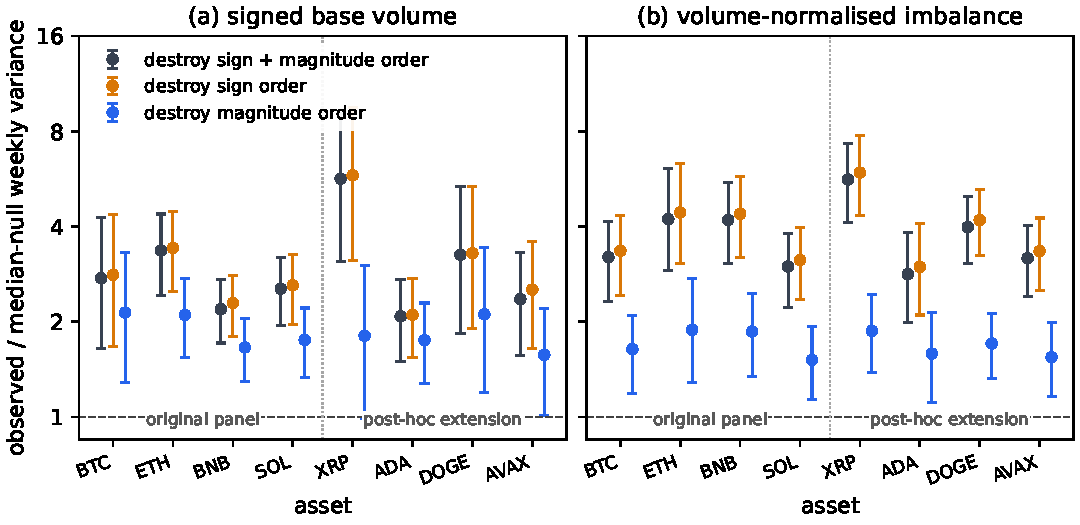
\includegraphics[width=0.98\textwidth]{../output/figuras/fig15_flow_null_decomposition.pdf}
  \caption{Weekly observed/null variance ratios for the joint, sign-order, and
  magnitude-order nulls under both flow definitions. Bars are eight-week
  moving-block bootstrap intervals; the transfer quantum cancels. Every joint
  ratio exceeds one, so the observed chronology carries variance that the
  calendar-matched memoryless histories do not. The two partial nulls motivate,
  but do not replace, the exact decomposition in Table~\ref{tab:decomp}.}
  \label{fig:counting}
\end{figure*}
\fi

\iffalse
% The following diagnostics are reported in the Supplemental Material. Keeping
% them out of the main narrative prevents consistency checks and benchmarks from
% competing with the empirical decomposition.
\section{Counting symmetry and second-order closure diagnostics}
\label{sec:identity}

This is a negative control, not a second empirical contribution. It asks
whether two apparently transport-like relations carry information beyond the
measured first two moments.

For completeness, define the finite-window asymmetry
\begin{equation}
  s(Q)=\ln\frac{P(Q_T=+Q)}{P(Q_T=-Q)} .
\end{equation}
We call its fitted linear slope $A$ an operational affinity. The name does not
make $Q_T$ an entropy production or $A$ a thermodynamic force. The conditions
under which a non-entropic current inherits a Gallavotti--Cohen symmetry are
restrictive \cite{barato2012}, and we do not establish them here.

A stronger limitation is algebraic. For a Gaussian variable with mean $m_T$
and variance $V_T$,
\begin{equation}
  s(Q)=\frac{(Q+m_T)^2-(Q-m_T)^2}{2V_T}
      =\frac{2m_T}{V_T}\,Q ,
  \label{eq:identity}
\end{equation}
exactly. The corresponding cumulant generator
$F_T(\chi)=\chi m_T+\chi^2V_T/2$ also obeys
$F_T(\chi)=F_T(-2m_T/V_T-\chi)$ identically. A measured straight line with
slope $2\avg{Q_T}/\Var(Q_T)$ is therefore consistent with a Gaussian null and
is not evidence for a nontrivial fluctuation theorem.

The measured affinity is far from the sign-randomised null in all eight
series, but only BTC and ETH retain its sign in all four consecutive temporal
blocks. At $T=16$ hourly candles, the measured values are
$A=-1.550\pm0.098$ for BTC and $-0.576\pm0.074$ for ETH. Across all windows,
$A$ follows $2\avg{Q_T}/\Var(Q_T)$ [Fig.~\ref{fig:affinity}]. The agreement is
a consistency check, not an independent closure.

The second-order counting variance is likewise fixed by the autocorrelation:
its direct value and the reconstruction from the sample $C_\eps$ differ by at
most $4.6\%$, with ratios $0.954$--$1.040$ over $64$ window--series
combinations. Deviations from Gaussianity are not absent. The cubic coefficient
of $s(Q)$ is $b_3=0.024\pm0.119$ for ETH$\cdot$1h and
$0.526\pm0.240$ for BTC$\cdot$1h at $T=16$, and the standardised third and
fourth cumulants do not converge uniformly to zero with $T$. We therefore
define no Gaussian crossover scale. The finite-window symmetry is retained as
a diagnostic, while the null-controlled variance and its exact decomposition
carry the empirical claim.

A conventional current large-deviation principle has speed $T$, whereas the
measured finite-window variance grows faster than $T$. We establish neither an
alternative speed nor a rate function. The log ratio above is consequently a
finite-window distributional statistic, not a demonstrated
Gallavotti--Cohen law.

\begin{figure*}[t]
  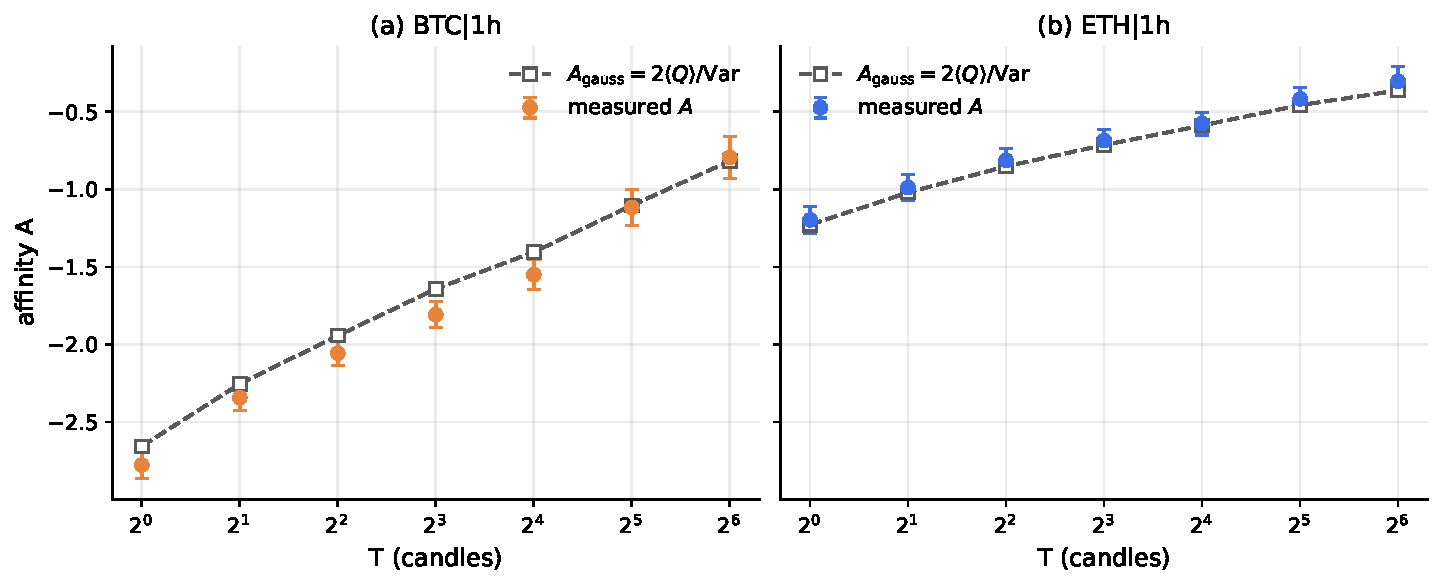
\includegraphics[width=0.92\textwidth]{../output/figuras/fig3_A_vs_Agauss.pdf}
  \caption{Measured affinity for the hourly BTC and ETH series against the
  Gaussian value $2\avg{Q_T}/\Var(Q_T)$ over dyadic counting windows.
  Agreement follows the Gaussian identity
  \eqref{eq:identity} and does not establish a fluctuation theorem.}
  \label{fig:affinity}
\end{figure*}

\section{Post-shock clocks as a negative control}
\label{sec:clocks}

We tested whether the two-time correlation ages after a market shock. Shocks
are returns above the $99.5$th percentile in absolute value, and the ensemble
contains $240$ hourly post-shock trajectories. The reliable result is
negative: the apparent ageing of the correlation is reproduced by randomly
placed events because the estimator is normalised by a pre-event quantity.

The mean normalised absolute return is compatible with an Omori-like
\cite{omori1894,lillo2003,zawadowski2006} profile, but the evidence does not
resolve an exponent. A fit
outside the initial fast regime gives the amplitude exponent
$\beta=0.61\pm1.01$, whose interval includes zero, and six of ten
asset--resolution fits terminate at an optimiser bound. We therefore use the
mean only to define the post-shock clock and make no claim of a universal
Omori law.

The measured correlation time appears to grow monotonically with waiting time,
with Spearman coefficient $+1.00$. The same analysis at randomly placed shocks
returns a median null coefficient of $+1.00$ [Fig.~\ref{fig:clocks}]. Dividing
the post-event signal by the volatility measured before the event introduces a
slow common factor as the volatility moves away from its initial value. That
factor produces an age profile even for a meaningless clock. The observed
growth is statistically indistinguishable from this placebo, so we report no
ageing of the correlation.

Ratio bias from a noisy denominator is well known
\cite{pearson1897,kronmal1993,ciuparu2016}, and event conditioning can amplify
measured correlations without changing the data-generating process
\cite{forbes2002,boyer1999}. A closely related effect occurs in a cooling
granular fluid, where normalised two-time correlations show full ageing in a
memoryless self-similar process and the effect disappears after proper
rescaling \cite{brey2007}. Our result has the narrower scope supported by the
data: for this event-conditioned estimator, random events reproduce the
measured age dependence. It does not exclude ageing under a different
observable or normalisation.

The same normalisation has appeared in aftershock and currency-crash analyses
\cite{abe2004,usmanova2017}. We do not reassess those data. Our result instead
supplies a general diagnostic: an event-conditioned two-time analysis that
normalises by a pre-event scale should include a randomly placed-event null
before interpreting an age profile.

\begin{figure*}[t]
  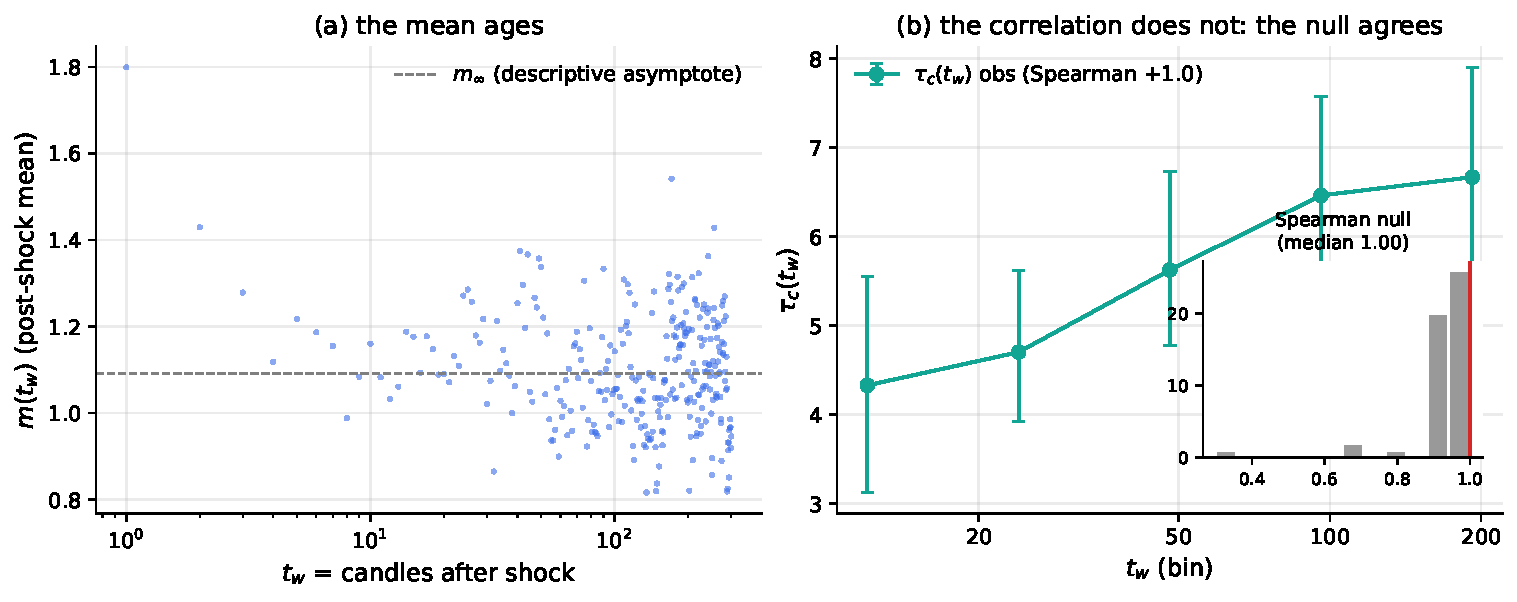
\includegraphics[width=0.90\textwidth]{../output/figuras/fig5_reloj_quench.pdf}
  \caption{Post-shock negative control for the pooled hourly primary panel.
  (a) The mean normalised absolute return relaxes with age, but its fitted Omori
  amplitude exponent is unresolved. (b) The correlation time appears to grow
  with age; randomly placed shocks reproduce the same monotone growth (inset),
  identifying the profile as an artefact of pre-event normalisation.}
  \label{fig:clocks}
\end{figure*}

\section{Statistical controls}
\label{sec:methods}

The central inference uses chronology-preserving measurements and
chronology-destroying nulls with identical preprocessing. Paired circular
moving-block bootstraps resample all terms of the decomposition together, so
the interval on the cross share retains their covariance. Positive synthetic
controls accompany the negative tests to distinguish absence of an effect
from an insensitive estimator. Full constructions, calibration results, and
robustness tables are given in the Supplemental Material \cite{supplement}.

Three checks determine how strongly we state the results. First, standard
Diebold--Mariano inference with Newey--West standard errors
\cite{diebold1995,neweywest1987} is unevenly calibrated under the observed heavy
tails: a nominal $5\%$ test rejects $4$--$6\%$ of null BTC samples but
$16$--$18\%$ of ETH samples. Second, a Westfall--Young maxT correction
\cite{westfall1993} over
$144$ predictive configurations gives a global $p=0.43$ even though the best
uncorrected cell has $p=2\times10^{-4}$. Third, synthetic persistent features
can correlate out of sample more strongly than the measured feature while
carrying no information. These controls motivate the empirical nulls used in
the main analysis; they are not additional market anomalies.

The memory estimators were calibrated on fractional Gaussian noise generated
by the Davies--Harte method \cite{davies1987}. The memory and counting exponents
are reported as finite-window estimates.
Four calibrated estimators disagree on the market data because the wavelet
log-scale diagram is not linear, rather than because one estimator fails on
known-input controls. Daubechies filters with one, two, and three vanishing
moments \cite{daubechies1992,percival2000} yield
$\nu=1.10$--$1.36$ and remove constant, linear, and quadratic mean drift,
respectively. The unfiltered block estimates are larger,
$\nu=1.31$--$1.43$. We therefore claim robust finite-window
superdiffusivity, $\nu>1$, but neither a unique asymptotic exponent nor a
resolved scale-dependent drift.

\section{Phenomenological response-field representation}
\label{sec:model}

\subsection{Response and an unresolved fluctuation--dissipation diagnostic}
\label{sec:response}

The lagged impact $R(\tau)$ is nearly flat in $\tau$, in sharp contrast to
$C_\eps$, which falls by roughly an order of magnitude over the same range
[Fig.~\ref{fig:base}(a)]. Fitting a log-slope to $R$ gives values scattered
around zero and small compared with $\gamma$ --- e.g.\ $b_R = 0.064\pm0.006$
(BTC$\cdot$1h) and $0.094\pm0.008$ (ETH$\cdot$1h) --- though we note honestly
that some series depart from flatness at resolvable significance
($b_R = -0.149\pm0.017$ for BNB$\cdot$4h). ``Flat'' here means flat to within
about a tenth of the decay exponent of the correlation, not flat exactly.

Flat response is what the surprise mechanism predicts
\cite{gerig2008,jaisson2014,muhlekarbe2026}: if the price integrates the
unpredictable part of the flow, the predictable part moves nothing and the
lagged covariance saturates immediately. We recover it as a check on our
conventions, not as a result.

One can formally construct the fluctuation--dissipation ratio
\begin{equation}
  \Teff(\tau) \;\equiv\; -\,C'_\eps(\tau)\big/R(\tau)
\end{equation}
but it differentiates a noisy sample autocorrelation and divides by an
estimated response. The finite-difference estimate does not propagate the
joint uncertainty, and the proposed single-exponent closure fails in all
eight series. We therefore make no empirical claim for $\Teff$.
Figure~\ref{fig:base}(b) is retained only to show that, with nearly flat
$R$, its shape is largely a transformed version of $C_\eps$, not an
independently resolved thermodynamic observable.

\begin{figure*}[t]
  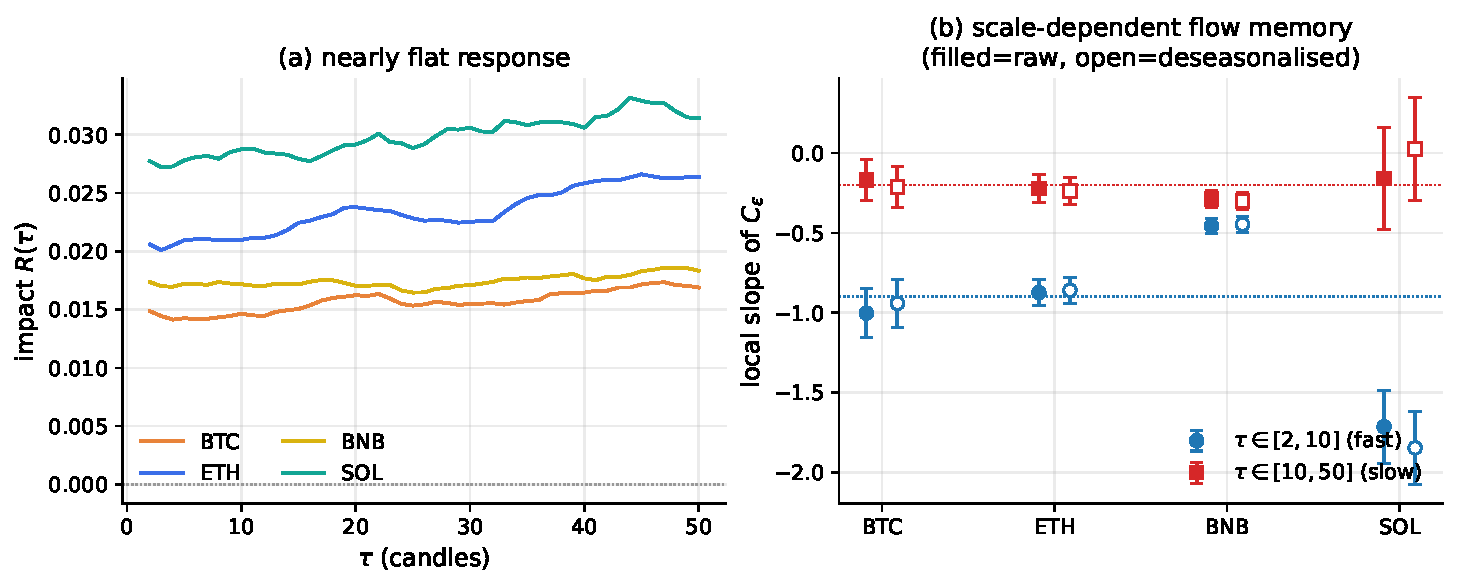
\includegraphics[width=0.98\textwidth]{../output/figuras/fig1_ceps_R_Teff.pdf}
  \caption{Base transport measurement for BTC, ETH, BNB, and SOL at hourly resolution.
  (a) The impact response is nearly flat in lag.
  (b) The raw fluctuation--dissipation diagnostic $\Teff(\tau)$; no inference
  is made from this derivative-based curve because its uncertainty is not
  identified and, with flat $R$, its shape is inherited from $C'_\eps$.
  (c) Local decay exponents of $C_\eps$ in the fast and slow windows, raw
  (filled) and deseasonalised (open); removing the daily cycle does not move
  them, so the slow regime is not the drive.}
  \label{fig:base}
\end{figure*}

We now encode the measured second-order structure in a minimal stochastic
response-field representation. The purpose is organisational, not microscopic: the action states which
relations follow once the correlation kernel and innovation coupling are fixed,
and therefore which observations cannot count as new evidence. Readers from
finance may view the construction as a compact generator of covariances and
cumulants; readers from physics should view it as a classical MSRJD representation
\cite{janssen1976,dedominicis1976}, not
as a quantum Keldysh contour for noncommuting market operators. The two
constructions share a doubled-field, two-time generating-functional structure
\cite{kamenev2011}. MSRJD path integrals have been used in finance for
derivative pricing under state-dependent noise \cite{rosaclot1999}. Here the
representation is applied to the measured signed-flow kernel and its response;
it organises the empirical closures but is not presented as a microscopic
derivation of market dynamics.

\subsection{The action}
\label{model:sec:action}

We use two fields, the signed flow $\eps(t)$ and the log-price $p(t)$, with
conjugate response fields $\epst$ and $\tilde p$, and statistical weight
$\propto e^{-S}$ with $S=S_\eps+S_p$.

\subsection{Flow sector}

The flow is a Gaussian field with a constant mean $\bar\mu$ and a stationary
memory kernel,
\begin{equation}
  S_\eps = \int\!\dd t\, \epst\bigl[\eps-\bar\mu\bigr]
         - \tfrac12\iint\!\dd t\,\dd t'\, \epst(t)\mathcal{K}(t-t')\epst(t') ,
  \label{model:eq:Seps}
\end{equation}
Integrating out $\epst$ along the imaginary
direction returns the Gaussian weight
$\exp\{-\tfrac12\iint(\eps-\bar\mu)\mathcal{K}^{-1}(\eps-\bar\mu)\}$, so that
\begin{align}
  G^K_{\eps\eps}(t,t')=\avg{\eps(t)\eps(t')}_c
  &=\mathcal{K}(t-t')=C_\eps(t-t'), \notag\\
  \avg{\eps\epst}&=\delta .
\end{align}

We deliberately do \emph{not} postulate a dynamics for $\eps$. The kernel is
measured, not derived, and its microscopic origin is not inferred here. Order
splitting is an established explanation for long-memory order signs
\cite{lillo2005,sato2023prl,sato2023prr}, but our aggregate candle data do not
identify it. Treating the flow as a prescribed non-Markovian bath keeps the
model honest about what it explains: the price coupling is the additional
modelling assumption, while the counting sector records consequences of the
supplied kernel and cannot provide independent evidence for it.

\subsection{Price sector}

The price integrates the \emph{innovation} of the flow rather than the flow
itself,
\begin{equation}
  S_p = \int\!\dd t\, \tilde p\bigl[\partial_t p-\lambda w\bigr]
      - \frac{D_p}{2}\int\!\dd t\, \tilde p^{\,2} ,
  \label{model:eq:Sp}
\end{equation}
where $D_p$ is the variance of price noise unrelated to flow and $w$ is defined
as follows. With $S_\eps(\omega)=\sum_k C_\eps(k)e^{-i\omega k}$ the flow
spectral density, positivity and $\int\ln S_\eps<\infty$ give the canonical
Wiener--Hopf factorisation $S_\eps(\omega)=\sigma_w^2|h(e^{-i\omega})|^2$ with
$h(z)=\sum_{k\ge0}h_kz^k$ causal, minimum-phase and $h_0=1$. Equivalently one
has the Wold representation \cite{wold1938,hamilton1994}
\begin{equation}
  \eps_t-\bar\mu=\sum_{k\ge0}h_k w_{t-k} ,
  \qquad \avg{w_tw_s}=\sigma_w^2\delta_{ts} ,
  \label{model:eq:wold}
\end{equation}
which defines the innovation $w_t$ as the part of $\eps_t$ not linearly
predictable from its strict past. The whitening filter $g=h^{-1}$ is causal, so
$w_t$ is a function of present and past flow and is orthogonal to the strict
past. The coupling in
Eq.~\eqref{model:eq:Sp} respects causality, as it must.

Equations \eqref{model:eq:Seps}--\eqref{model:eq:Sp} are the entire model. Everything below
is a consequence.

\subsection{Why the response is flat}
\label{model:sec:flat}

\begin{proposition}[Flat impact]
\label{model:prop:flat}
Under Eqs.~\eqref{model:eq:Sp}--\eqref{model:eq:wold}, the lagged impact
\begin{equation}
  R(\tau)\equiv\frac{\mathrm{cov}(p_{t+\tau}-p_t,\eps_t)}{\Var(\eps)}
\end{equation}
is independent of $\tau$ for all $\tau\ge1$, with
$R(\tau)=R_0=\lambda\sigma_w^2/\sigma_\eps^2$.
\end{proposition}

\begin{proof}
From Eq.~\eqref{model:eq:Sp}, $p_{t+\tau}-p_t=\lambda\sum_{s=t}^{t+\tau-1}w_s$ plus
noise uncorrelated with $\eps$. Equation \eqref{model:eq:wold} gives
$\mathrm{cov}(w_s,\eps_t)=\sigma_w^2h_{t-s}\mathbf1\{s\le t\}$. In the sum $s$
runs over $\{t,\dots,t+\tau-1\}$, so only $s=t$ survives, contributing
$\sigma_w^2h_0=\sigma_w^2$. Hence $\mathrm{cov}=\lambda\sigma_w^2$ for every
$\tau\ge1$, independent of $\tau$.
\end{proof}

The mechanism --- the price responds to the surprise in the flow, so the
predictable part of a persistent flow moves no price and prices stay nearly
martingale --- is not ours. It is the standard resolution of the
persistence-versus-martingale puzzle \cite{gerig2008,jaisson2014,muhlekarbe2026},
and it also removes the need for a decaying propagator to reconcile correlated
flow with uncorrelated returns \cite{bouchaud2004,bouchaud2018}. We recover it
here as a check that the bookkeeping in Eqs.~\eqref{model:eq:Seps}--\eqref{model:eq:Sp} is
right. Its value is what it enables next: with $R$ pinned flat, the
fluctuation--dissipation ratio has no shape freedom left.

\begin{remark}
The measured response is flat to within about a tenth of the decay exponent of
the correlation, not flat exactly; some series depart from flatness at
resolvable significance \cite{code_keldysh_finance}. Proposition~\ref{model:prop:flat} is the
idealisation, and the residual slope is a measure of how far real flow departs
from the pure-innovation coupling.
\end{remark}

\subsection{A formal fluctuation--dissipation diagnostic}
\label{model:sec:teff}

The representation permits the formal ratio
\begin{equation}
  \Teff(\tau)\equiv-\frac{C'_\eps(\tau)}{R(\tau)}
  \simeq-\frac{C'_\eps(\tau)}{R_0}.
  \label{model:eq:teff}
\end{equation}
Because the response is nearly flat, this curve inherits its shape from the
measured correlation and contains no independent second-order information.
Differentiating a noisy correlation and dividing by an estimated response
would require joint uncertainty propagation, which the finite-difference
diagnostic does not provide. Its proposed single-exponent form fails in all
eight series. We therefore use Eq.~\eqref{model:eq:teff} only to state what
the phenomenological representation would imply and make no empirical
effective-temperature claim.

\subsection{The counting sector}
\label{model:sec:counting}

Let $Q_T=\sum_{t=1}^{T}\eps_t$ be the flow transferred in a window of $T$
candles. Introducing the counting field $\chi$ conjugate to $Q_T$ --- the object
carrying opposite signs on the two contour branches, as in the counting
statistics of mesoscopic transport
\cite{levitov1993,levitov1996,schoenhammer2007,esposito2009} --- the cumulant
generating function is $F_T(\chi)=\ln\avg{e^{\chi Q_T}}$. For the Gaussian
action \eqref{model:eq:Seps} it truncates exactly at second order,
\begin{equation}
  F_T(\chi)=\chi m_T+\tfrac12\chi^2V_T ,
  \quad
  V_T=\Var(Q_T)=\!\!\sum_{t,t'=1}^{T}\!\!C_\eps(t-t') ,
  \label{model:eq:cgf}
\end{equation}
so every cumulant $\kappa_n$ with $n\ge3$ vanishes identically. The relation
$V_T=\sum_{t,t'}C_\eps(t-t')$ is exact when both sides use the same covariance
estimator and windows. Our direct non-overlapping-window estimate and the
reconstruction from a separately estimated full-series covariance differ by
at most $4.6\%$ over $64$ window--series combinations. That discrepancy is a
finite-estimator consistency check, not independent empirical confirmation
\cite{code_keldysh_finance}.

Equation~\eqref{model:eq:cgf} immediately gives the Gaussian affinity
identity derived in Sec.~\ref{sec:identity}. We do not repeat the proof here.
The conclusion is the same in both languages: the measured linear symmetry
and the reconstructed variance are consequences of the second-order closure,
not independent evidence for a fluctuation theorem or for the
response-field representation. Higher cumulants and resolved departures from
linearity are the quantities that can test the Gaussian approximation.

\subsection{Finite-window scaling implied by the kernel}
\label{model:sec:crossover}

For a single power-law kernel $C_\eps(\tau)=A\tau^{-a}$ with $0<a<1$,
\begin{equation}
  V_T\simeq\frac{2A}{(1-a)(2-a)}\,T^{\,2-a},
  \qquad \nu=2-a .
  \label{model:eq:varscaling}
\end{equation}
At $a=1$ the leading form is $T\log T$, while a summable kernel with $a>1$
is generically asymptotically diffusive when its integrated covariance is
nonzero; exact cancellation can remove the linear term. The mapping is therefore conditional on the
exponent and cannot be applied indiscriminately to the fast fitted regime.

If $\avg{Q_T}=\bar\mu T$, the Gaussian identity also gives the exact
finite-scale relation
\begin{equation}
  \frac{A_{T_2}}{A_{T_1}}
  =\frac{T_2}{T_1}\frac{V_{T_1}}{V_{T_2}} .
  \label{model:eq:Aexact}
\end{equation}
This relation contains no dynamical information beyond the measured moments,
so its agreement with the stable-affinity series is another consistency check.

A two-component empirical kernel can produce a drifting local slope, but the
data do not establish that drift independently. The block estimator is
sensitive to the measured mean drift, whereas filters with up to three
vanishing moments retain global finite-window superdiffusivity and do not
resolve a monotone crossover at the longest windows. Detailed bands,
calibration tests, and the estimator comparison are reported in the
Supplemental Material \cite{supplement}. We therefore retain only the robust
statement $\nu>1$ over the measured windows and make no asymptotic or
two-regime scaling claim.

\section{An exactly controlled mesoscopic benchmark}
\label{model:sec:device}

The phenomenological representation does not supply a microscopic market
model. We therefore use a separate, exactly controlled conductor only as a
benchmark for the transport language. The device is a noninteracting level
between two leads, driven by a bias quench and coupled to a wide Lorentzian
band plus a narrow band of width $W$ \cite{jauho1994,levitov1996,blanter2000}.
Its nonequilibrium Green functions and counting statistics are computed with
an independent solver \cite{code_qteom}.

The structured bath produces two relaxation regimes in the mean current,
whereas a single wide band produces one. Its post-quench retarded Green
function remains time-translation invariant, and the measured correlation
time is $\tau_c=3.375$ at all eight waiting times and in every bath
configuration. The device therefore demonstrates that a relaxing mean can
coexist with a non-ageing correlation without an age-dependent kernel. It
does not establish that the market has the same microscopic dynamics.

The counting comparison is deliberately structural. The device has
$\mathcal F=0.332$--$0.341$ under the conventional mesoscopic normalisation
and finite-window variance slopes $0.94$--$0.99$. The market uses
heterogeneous classical transfers, so its absolute Fano normalisation is not
comparable to the fermionic one. What can be compared is the scaling: the
finite-memory device is diffusive, while the market remains superdiffusive
under drift-resistant estimators and exceeds its memory-destroying temporal
nulls [Fig.~\ref{model:fig:device}].

A fixed-window exponential fit to the device transient can itself develop an
apparent maximum even though the exact pole rates remain smooth. That
estimator effect is analysed in the companion Letter \cite{paper3_letter};
here it serves only as a warning that fitted rates need not be physical
modes. Thus the conductor calibrates the interpretation of response, memory,
and counting statistics without transferring a fermionic bound or a
microscopic mechanism to the market.

\begin{figure*}[t]
  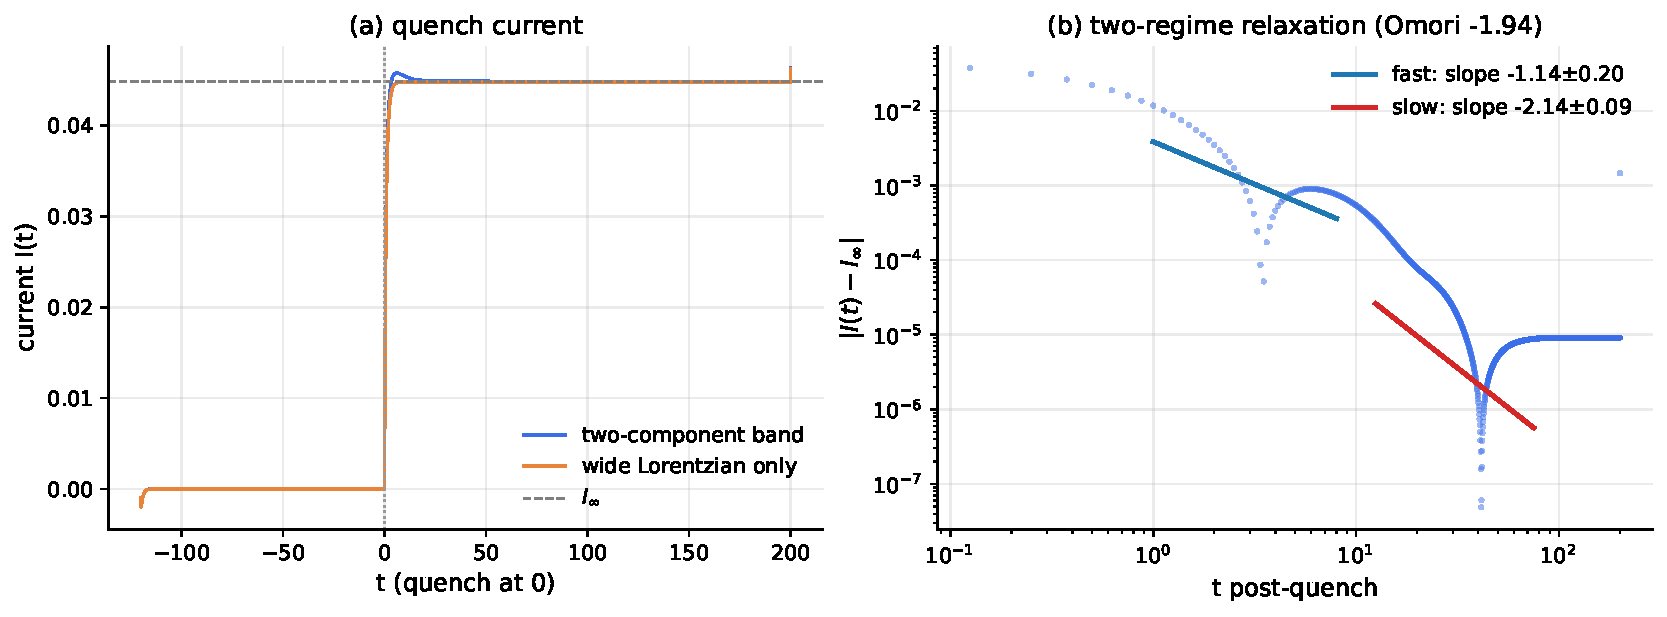
\includegraphics[width=0.94\textwidth]{../output/figuras/fig7_quench_current.pdf}
  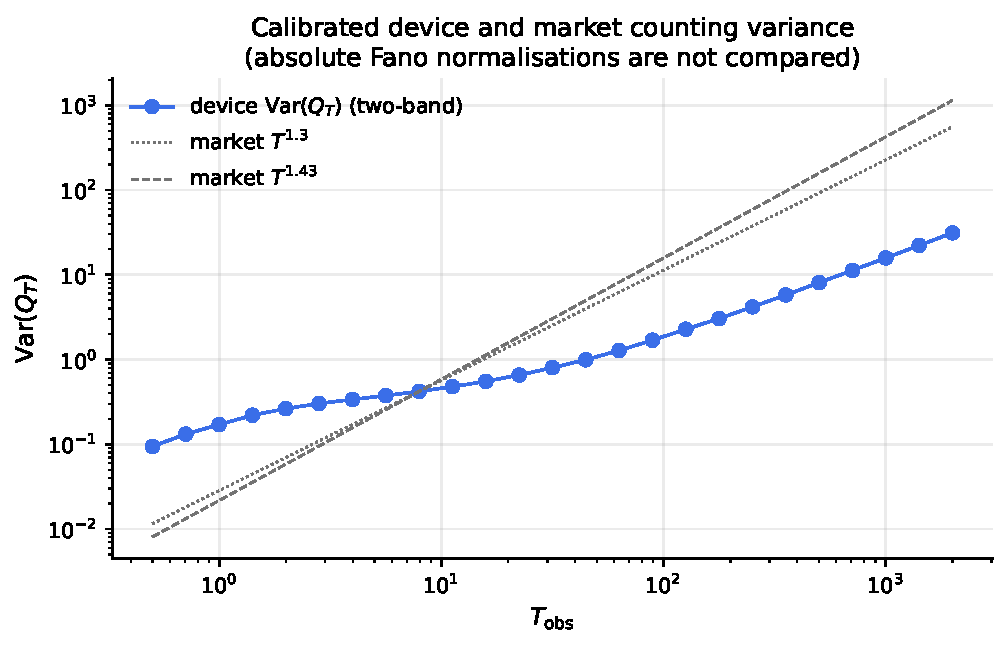
\includegraphics[width=0.68\textwidth]{../output/figuras/fig8_varQ_dispositivo_vs_mercado.pdf}
  \caption{Exactly controlled transport benchmark. (a) Current after the bias
  quench. (b) A structured bath produces two mean-relaxation regimes, whereas
  a single wide band produces one. (c) The finite-memory device has diffusive
  counting variance; the market band shows finite-window superdiffusive
  growth. The comparison concerns scaling, not the unlike absolute Fano
  normalisations.}
  \label{model:fig:device}
\end{figure*}

\fi

\section{Ancillary scope controls}

The Supplemental Material \cite{supplement} records three checks that delimit
the central result. First, a linear finite-window symmetry has the exact
Gaussian explanation fixed by the first two moments. Second, apparent
post-shock ageing is reproduced by randomly placed events under the same
pre-event normalisation. Third, a phenomenological response-field construction
and a noninteracting transport benchmark provide consistency checks, not a
microscopic market theory or additional empirical evidence.

\section{Discussion and conclusions}
\label{sec:integrated-discussion}

\paragraph*{Established.}
Chronology contributes counting variance beyond calendar-matched one-point
statistics under both flow definitions. Equations~\eqref{eq:decomp} and
\eqref{eq:reccorrection} partition that excess exactly. Within it, the
corrected sign--size cross contribution exceeds the sign-memory contribution
in all eight primary point estimates, while paired bootstrap intervals
establish a majority share in six. This partition component is not an
identified causal coupling.
The per-stratum reference and its explicit recentring correction are fixed by
the operational stratified null, not chosen to maximise that term. The same analysis establishes
finite-window superdiffusivity under drift-resistant estimators, without
determining an asymptotic exponent.

\paragraph*{Limits.}
The failed predeclared all-assets gate is not replaced by the post-hoc
extension, and cross-asset correlations preclude treating the four primary
assets as independent replications. The exact partition does not identify a
causal coupling: its cross term includes the product of marginal memories as
well as any nonfactorisable sign--size synchrony. It also has the declared
scope of public candle aggregates from one venue, not individual parent orders
or a population of market structures. Supplementary controls show why neither
a finite-window symmetry, a post-shock clock, nor a phenomenological transport
analogy should be promoted to a separate market mechanism.

What remains is a compact empirical statement: relative to a calendar-matched
temporal null, chronology amplifies finite-window counting fluctuations, and
an exact null-aligned partition assigns a larger sign--size cross contribution
than sign-memory contribution to the excess in all eight primary point
estimates, with a majority resolved in six. Establishing a universal majority,
an asymptotic scaling exponent, or a microscopic mechanism requires different
data and tests.

\section*{Data Availability}
The market records used here are public Binance candle and trade archives. A
versioned release of the analysis code, data provenance, and numerical outputs
is available in Ref.~\cite{code_keldysh_finance}; the independent transport
solver is available in Ref.~\cite{code_qteom}.

\begin{acknowledgments}
OpenAI Codex (GPT-5, accessed August--September 2026) was used for code
assistance, numerical cross-checks, literature organisation, and language
revision. The authors specified the tasks, verified the derivations and
numerical outputs against the deposited code and data, and take responsibility
for the content.
\end{acknowledgments}

\bibliographystyle{apsrev4-2}
\bibliography{refs}
\end{document}
